\documentclass[a4paper,12pt]{article}

\usepackage{Packages}
\usepackage{subfigure}
\usepackage{amsmath}


\begin{document}
\begin{titlepage}

\begin{center}

% Upper part of the page. The '~' is needed because \\
% only works if a paragraph has started.

\includegraphics[width=0.6\textwidth]{./Figures/TUe}~\\[2cm]


%\vspace*{10cm}

% Title
\HRule \\[0.4cm]
{ \huge \bfseries 2IMM20 - Foundations of datamining\\[0.3cm] }
\HRule \\[1.5cm]
\textbf{Assignment 2}


% Author and supervisor

\vfill

\begin{table}[h]
\begin{tabular}{ll}
\textbf{Students:} & \\
Joris van der Heijden & (0937329)\\
Bram van der Pol & (0780042)\\

\\
\textbf{Email addresseses:} & \\
j.j.m.v.d.heijden@student.tue.nl \\
a.f.v.d.pol@student.tue.nl \\
\\
\textbf{Supervisors:} &\\
Dr.ir. Joaquin Vanschoren
\\

%\textbf{Supervisors:} & \\
%Dr. M.Holenderski \\
\end{tabular}
\end{table}



% Bottom of the page
\large
{ Eindhoven, \today}

\end{center}


\end{titlepage}
 %included in part 1

\tableofcontents %included in part 1

\section{A data mining challenge}
This sections shows the steps that are done to improve the model for the datamining challange. This is done in a small report to show the different steps with the generated figures. 

\subsection{Detects accents in speech data}
First three previously used models are fitted on the data to check which model works best in this case.

\begin{figure}[H]
\hfill
\makebox[\textwidth][c]{{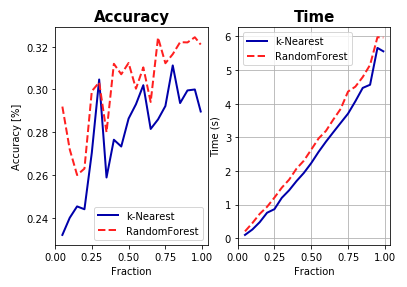
\includegraphics[width=12cm]{./Figures_2/Which_algorithm.png}}}
\hfill
\caption{Performance of the k-Nearest and Random forest algorithms. }
\label{Q41a}
\end{figure}

The RandomForest classifier is chosen because this gives the best accuracy with the default parameters. The computing time for both algorithms is almost equal for bot algorithms. The logistic regression (not shown) has a large computation time with low performance, so therefore this model is not chosen. \\
In order to save computation time chosen is to start with a coarse grid and make this mesh finer and finer to come to the optimal solution. The grid search is done for only 1\% of the data to save computing time. After the optimal solution is found the model is fitted on the entire data set using the obtained hyperparameters. The coarse grid search for 1\% if the data is shown is figure \ref{}. 

\begin{figure}[H]
\hfill
\makebox[\textwidth][c]{{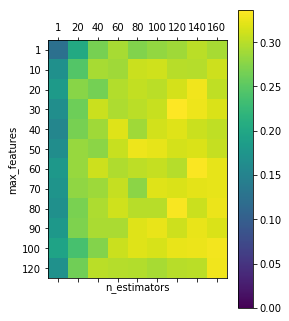
\includegraphics[width=12cm]{./Figures_2/features_30_estimators_120.png}}}
\hfill
\caption{A coarse grid search for 1\% of the data with the Random Forest classifier. The optimal parameters are: $n_{estimators}=120$ and $max{features}=30$}
\label{Q41b}
\end{figure}

Now we ran a finer grid search near the domain  $n_{estimators}=120$ and $max{features}=30$. The results is shown in figure \ref{Q41c}
\begin{figure}[H]
\hfill
\makebox[\textwidth][c]{{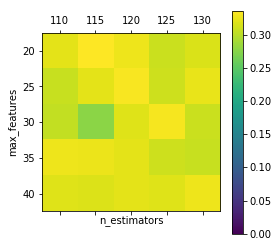
\includegraphics[width=12cm]{./Figures_2/features_30_estimators_115_score_0_34.png}}}
\hfill
\caption{A coarse grid search for 1\% of the data with the Random Forest classifier. The optimal parameters are: $n_{estimators}=115$ and $max{features}=30$. This gave a score of 0.34 (for 1\% of the data)}
\label{Q41c}
\end{figure}
Now we ran the model with the obtained parameters and achieved a score shown in figure \ref{Q41d}.


\begin{figure}[H]
\hfill
\makebox[\textwidth][c]{{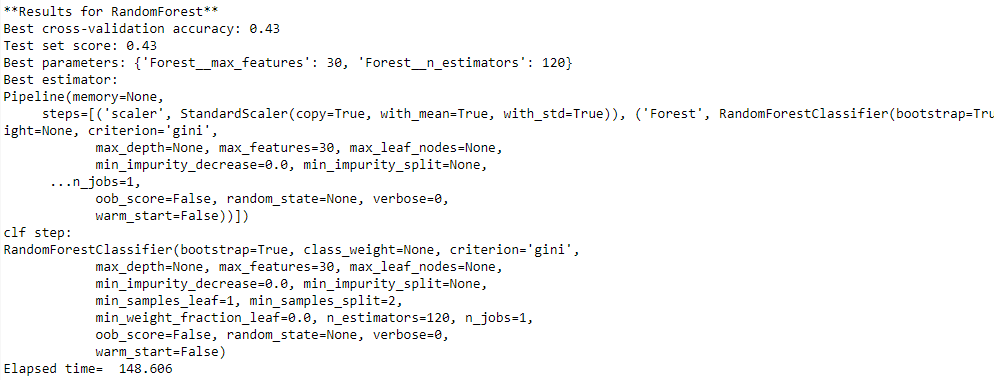
\includegraphics[width=12cm]{./Figures_2/Achieved_score.png}}}
\hfill
\caption{RandomForest score for: $n_{estimators}=115$ and $max{features}=30$. This gave a score of 0.43 for 100\% of the data}
\label{Q41d}
\end{figure}

In order to improve the results, the leaderboard was checked to look for the best algorithm. This was the $Keras$ classifier and therefore decided was to use this neural network API. Unfortunately this model took too much time to run, and therefore the optimization of the Keras algorithm did not have the desired outcome. 


\end{document}
